%%%%%%%%%%%%%%%%%%%%%%%%%%%%%%%%%%%%%%%%%
% University/School Laboratory Report
% LaTeX Template
% Version 3.1 (25/3/14)
%
% This template has been downloaded from:
% http://www.LaTeXTemplates.com
%
% Original author:
% Linux and Unix Users Group at Virginia Tech Wiki 
% (https://vtluug.org/wiki/Example_LaTeX_chem_lab_report)
%
% License:
% CC BY-NC-SA 3.0 (http://creativecommons.org/licenses/by-nc-sa/3.0/)
%
%%%%%%%%%%%%%%%%%%%%%%%%%%%%%%%%%%%%%%%%%

%----------------------------------------------------------------------------------------
%	PACKAGES AND DOCUMENT CONFIGURATIONS
%----------------------------------------------------------------------------------------

\documentclass{article}

\usepackage{siunitx} % Provides the \SI{}{} and \si{} command for typesetting SI units
\usepackage{graphicx} % Required for the inclusion of images
\usepackage{natbib} % Required to change bibliography style to APA
\usepackage{amsmath} % Required for some math elements 

\setlength\parindent{0pt} % Removes all indentation from paragraphs

\renewcommand{\labelenumi}{\alph{enumi}.} % Make numbering in the enumerate environment by letter rather than number (e.g. section 6)

%\usepackage{times} % Uncomment to use the Times New Roman font

%----------------------------------------------------------------------------------------
%	DOCUMENT INFORMATION
%----------------------------------------------------------------------------------------

\title{Dynamic Connect-4 \\ Assignment 1 \\ Artificial Intelligence - ECSE526} % Title

\author{Otis \textsc{Samuel}} % Author name

\date{\today} % Date for the report

\begin{document}

\maketitle % Insert the title, author and date

\begin{center}
\begin{tabular}{l r}
Instructor: Jeremy Cooperstock % Instructor/supervisor
\end{tabular}
\end{center}

% If you wish to include an abstract, uncomment the lines below
% \begin{abstract}
% Abstract text
% \end{abstract}

%----------------------------------------------------------------------------------------
%	SECTION 1
%----------------------------------------------------------------------------------------
\section{Introduction}
This report shows the implementation of minimax and alpha-beta algorithms in the context of an adversarial game. The game is a custom version of Connect-4. In this version, Dynamic Connect-4, a 7x7 board has 6 tokens for white and 6 tokens for black disposed on the board, as per figure\ref{fig:dc4}. The goal is for the player to align four of his tokens in diagonal, a row or a column. Following this objective, we will compare minimax and alpha-beta pruning across specific performance metrics. One of these is the number of nodes openend according to the depth cutoff, that is, the numbder of possible states depending on the depth in which we go in the search-tree of the minimax function. Another metric is the tradeoff between the complexity of the heuristic function, which attributes a more or less "desireable" value to each states, and the depth at which we search. Other specifics about this assignment will be discussed as per the criterions that were given for this assignment.
	\begin{figure}
		\hfill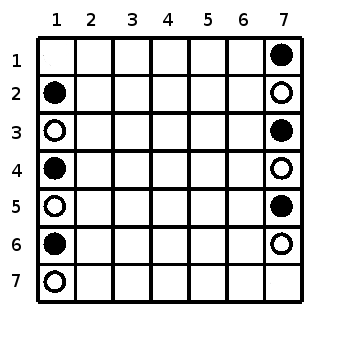
\includegraphics[height=3.5cm]{dyncon4.png}\hspace*{\fill}
		\caption{ Dynamic Connect-4 board with white and black tokens on starting positions}
		\label{fig:dc4}
	\end{figure}
	
\newpage
\section{Minimax and AlphaBeta Nodes vs. Depth Cutoffs}

This section of the report shows the graphs nodes/depth cutoffs of each given configuration of the board. For each of them, we explore a number of expanded nodes at different depth level. This helps to compare and realize the necessity of implementing alpha-beta pruning in adversarial games.
	\begin{figure}[!b]
		\hfill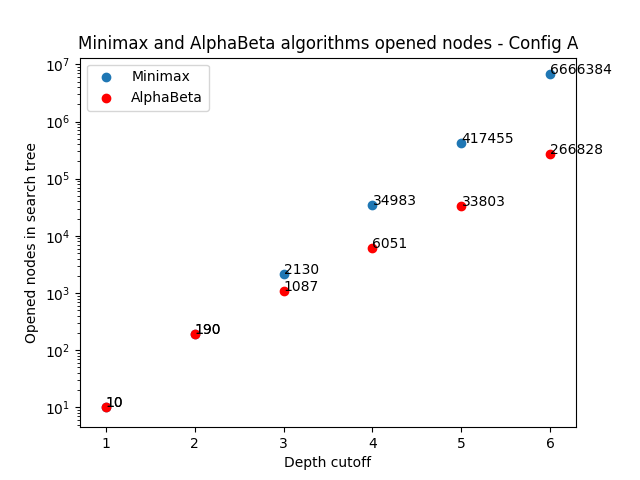
\includegraphics[height=8cm]{configA_nodes_depth.png}\hspace*{\fill}
		\caption{ Expanded nodes versus depths cutoffs for configuration A}
		\label{fig:nodesA}
\newpage
	\end{figure}
		\begin{figure}
		\hfill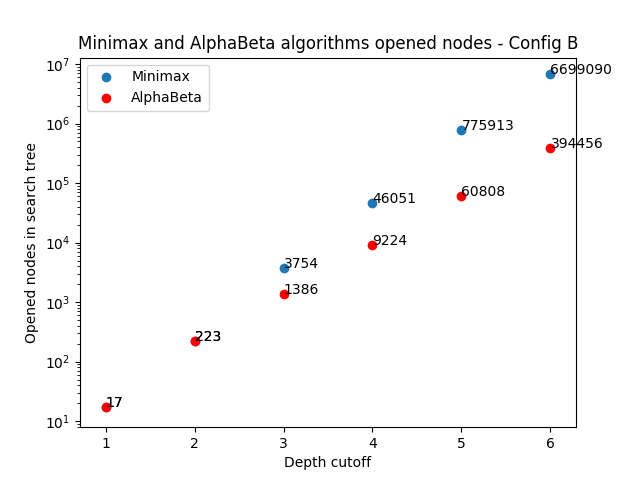
\includegraphics[height=8cm]{configB_nodes_depth.png}\hspace*{\fill}
		\caption{ Expanded nodes versus depths cutoffs for configuration A}
		\label{fig:nodesB}
	\end{figure}
		\begin{figure}
		\hfill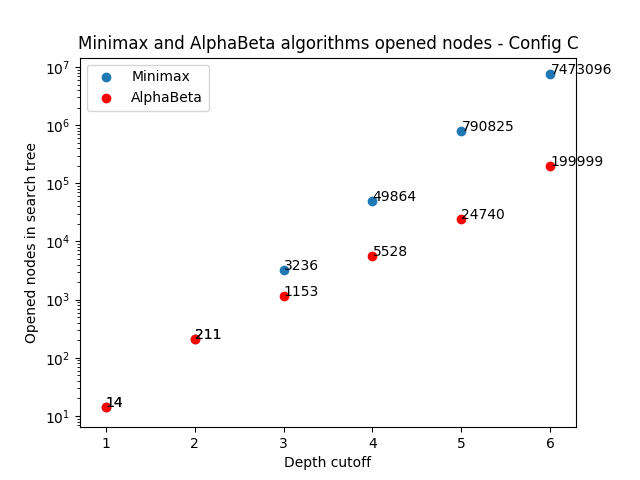
\includegraphics[height=8cm]{configC_nodes_depth.png}\hspace*{\fill}
		\caption{ Expanded nodes versus depths cutoffs for configuration A}
		\label{fig:nodesC}
	\end{figure} 
As we clearly see in figures \ref{fig:nodesA}, \ref{fig:nodesB} and \ref{fig:nodesC}, a minimax search search-tree expands dramatically fast with an exponential growth, thus the need for a logarithmic scale. It is possible to see the exact number of visited nodes by each algorithms beside the points in each graph. Moreover, we see the alpha-beta pruning giving excellent results and tremendously reducing the number of nodes being visited. This means that we can go deeper for a given time with alpha-beta than with a normal minimax algorithm. From these results, we can estimate the number of nodes visited is \[nodes = O(b^d) \] where b is the branching factor, or number of moves at each game state and d is the depth cutoff. In this context, the number of move at each state was averaged on 34 consecutive moves. This showed an average of 12.25 possible moves per state with a standard deviation of 2.25. Thus, we can estimate, for this game, the following function : \[nodes = O(12.25^d) \]. On the other hand, we see that, for alphabeta pruning, the number of nodes visited becomes \[nodes = O(12.25^{d/2}) \], at best and \[nodes = O(12.25^d) \] at worst. This is easily explanable by examining how alpha beta pruning works. Alpha-beta will cut parts of the tree when it sees that this is the best move the opponent can do for this subtree. However, if after each player's turn the opponents moves were ordered from best to worst, alpha-beta would cut the rest of the tree. The nodes visited would then become 8*1*8*1*8*...This shows that alpha-beta drastically cuts in the number of nodes visited. If we look at the comparisons of table \ref{table:performance_results}, we see that, the deeper we go in the search-tree, the more alpha-beta is efficient at cutting unvaluable nodes. 
All these reasons help to show that alpha-beta is much more efficient than minimax at finding the best move in a search-tree for an adversarial game.

\begin{table}[ht]
		\centering
		 \begin{tabular}{cccc} 
		 \hline
		 Ply & Minimax nodes & Alpha-beta nodes & Reduction of search-space \\ [0.5ex] 
		 \hline\hline
		 3 & 3236 & 1153 & 64.37\% \\
		 \hline
		 4 & 49864 & 5528 & 88.91\% \\
		 \hline
		 5 & 790825 & 24740 & 96.87\% \\
		 \hline
		 6 & 7473096 & 199999 & 97.32\% \\
		 \hline
		\end{tabular}
		\label{table:performance_results}
		\caption{Performance of algorithms on configuration C}
		\end{table}

\section{Alphabeta and moves ordering}
In this section, we look at the differences in performance when we use a different way of generating the order of the moves. The first method implemented in this project order moves starting at the top left corner of the board and reads each cells from left to right by going down, as seen in figure \ref{fig:movesleftright}. If the cell is occupied by the player's token, it attributes moves in a N, S, E, W order. 
We try two other methods to validate the effect of move generation. The first method take the same move generator, but then shuffles all the moves in the generated array.
The other method uses the evaluation function to directly attribute a score to each possible move and then orders the list from best to worst move for this player at this depth.
	\begin{figure}
		\hfill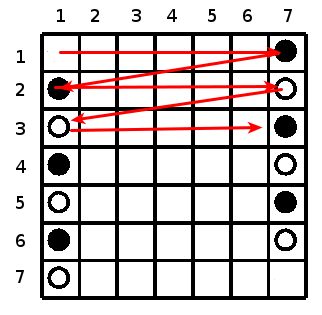
\includegraphics[height=8cm]{movesleftright.png}\hspace*{\fill}
		\caption{ Move generator}
		\label{fig:movesleftright}
	\end{figure}
	\begin{figure}
		\hfill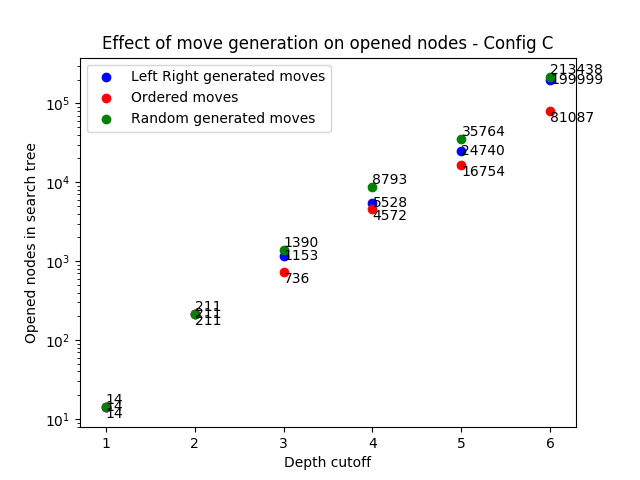
\includegraphics[height=8cm]{all_gen_moves.png}\hspace*{\fill}
		\caption{ Move generator}
		\label{fig:movesrand}
	\end{figure}
	
As figure \ref{fig:movesrand} shows it, if we shuffle all the moves, the number of nodes visited by alpha-beta changes from the normal method used. Even though the number of visited nodes never changed for configuration C with multiple session with the same move generator, it changed as soon as the move list was reordered. However, shuffling would have more or less the same impact on the number of visited nodes depending on the board configuration. This is because there is no "special" order attributed to the moves when we use left-right and shuffling generation. An interesting phenomenon appeared when using sorting to generate the moves. The number of visited nodes went down fast. This happens because alpha-beta breaks as soon as it judges that a leaf or a sub-tree will not produce a good move, that is, outside the alpha and beta boundaries. What happens here is that, at each level, once the first moves have been calculated, alpha-beta cuts most of the tree because we already have the best moves in order. However this is not giving best results because the evaluation function, as it is now, cannot perfectly judge if the visited state is enough a good state to lead to a victory. Still, it greatly diminishes the uncertainty on the quality of the move. Thus, we can assume that, theoretically, if the moves were to be all sorted from best to worst at each player's turn, we would have the best possible performance of alpha-beta pruning, as seen in this equation: \[nodes = O(12.25^{d/2}) \] 
Sadly, sorting all the moves would take so much time that it is not an acceptable behavior for an adversarial game.
	
 
%----------------------------------------------------------------------------------------
%	SECTION 2
%----------------------------------------------------------------------------------------

\section{Heuristic function}
This section explains the choice of the evaluation function and its underlying heuristics.
A simple evaluation function was used in determining scores for possibles states. Considering that an endgame score of [-100, 100] was attributed for a winning max or min player, scores of [-70, 70] were given for moves that gave a three-tokens-in-a-row for max and min players, be it in a row, a columnor a diagonal. For moves that gave two-tokens-in-a-row, attributed scores were [-30, 30]. The last heuristic used was a gaussian distribution of the usefulness of each square, as per figure \ref{fig:gaussian}. This heuristic, in itself, only assumes that a center position on the board is better. Used with the precedent heuristics, it also helps distinguish between moves that may the same in terms of goodness. This set of heuristics is very simplistic, thus taking less time to evaluate each move and giving more time for deeper search in the minimax tree. Moreover, the scores given by the gaussian distribution are lower than other heuristics to avoid a power-play were the pieces only strive to reach the middle.

	\begin{figure}[!b]
		\hfill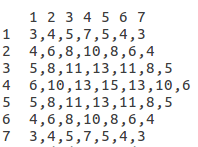
\includegraphics[height=3cm]{gauss_distrib.png}\hspace*{\fill}
		\caption{ Gaussian scoring distribution of each square of the board}
		\label{fig:gaussian}
	\end{figure}

%----------------------------------------------------------------------------------------
%	SECTION 3
%----------------------------------------------------------------------------------------

\section{Computational tradeoffs}
As wee have seen in the past sections, the number of visited nodes in a search-tree tends to grow exponentially, thus consuming a lot of time and a lot fo memory. Considering that, even with alpha-beta pruning we have the following performances :
Visited nodes :
\[nodes = O(12.25^{d/2}) \] at best and \[nodes = O(12.25^{d}) \] at worst

This means that the memory consumption will also grow exponentially, eventually hitting a wall in the system's memory capacity. 

On the other hand, if we have a complex evaluation function, it will take more time to visit a node. In a context of time-constrained adversarial play, this will greatly diminish the depth at which we dive to evaluate the best move, thus increasing the horizon effect. The horizon effect is a problem in artificial intelligence because the agent will take the best assumed move at a given depth, when this move could in fact be the worst to do if we went a bit deeper in the search tree. Thus it would be best to visit more nodes to mitigate the horizon effect. Some algorithms exist to mitigate this effect by examinig specifics good move beyond the depth cutoff. This is called a quiescent search. However this algorithm was not used in this project. In this context, a simple heuristic was used to search deeper in the given time-limit of the games. 





%----------------------------------------------------------------------------------------
%	SECTION 4
%----------------------------------------------------------------------------------------

\section{Conclusion}
This project has seen the implementation of a minimax algorithm as well as the alpha-beta pruning method. We could derive important performance metrics from the results of these algorithms. First, it is important to note that the number of nodes visited by the minimax algorithm grows exponentially extremely fast. This poses problem in terms of memory consumption and limited time allowed to decide the best move to make in an adversary play. Thus, the alpha-beta pruning showed excellent results in reducing the number of nodes visited. 
An important parallel was drawn between the order in which moves are generated and visited nodes. We saw that a move sorting from good to bad would greatly improve the performance of alpha-beta pruning. 
Moreover, we saw that the complexity of the evaluation function increases the time spent in each node of the search-tree, thus decreasing the total number of visited nodes when we increase complexity of the heuristics in the evaluation function. A simpler function will allow us to go deeper in the search tree. However, a well designed evaluation function could permit the best tradeoff between complexity and depth of the tree. A tree a bit more shallow and very good heuristics could lead to even better results than sole depth of the move search.
An interesting and different take on this project would be to use the "openai" platform and develop a gym environment where a neural network (NN) such as Pytorch or Tensorflow could be trained by reinforcement learning. It has been proven lot of times with much more complex games that this environment is user friendly and gives good result fast. The only goal would be to define a good environment with well-adjusted rewards for the NN.


\end{document}
